% Preamble
\documentclass{article}
\usepackage[left=1in, right=1in, top=1in, bottom=1in]{geometry}

% packages
\usepackage {lmodern}
\usepackage [T1]{fontenc}
\usepackage {amsmath}
\usepackage {amssymb}
\usepackage {amsfonts}
\usepackage {graphicx}
\usepackage {fullpage}
\usepackage {gensymb}
\usepackage {caption}
%\usepackage{nopageno}
\usepackage {cite}
\usepackage {setspace}
\usepackage [version=4]{mhchem}
\usepackage {multicol} 
\usepackage {sectsty}
\usepackage {textcomp}

% graphics path
\graphicspath {{images/}}

% bibliography style 
\bibliographystyle{unsrt}    

% font settings
	%%% headings font
	\sectionfont{\fontfamily{ptm}\fontsize{12}{15}\selectfont} 
	\subsectionfont{\fontfamily{ptm}\fontsize{10}{12}\selectfont}

	%%% paragraph font
	\usepackage{fontspec}
	\defaultfontfeatures{Mapping=tex-text, Scale=MatchLowercase}
	\setmainfont{Arial}

% Title
\title{An Investigation of Electrochemistry \\
Using Chronoamperometry \& Cyclic Voltammetry}

\author{{Justin Chao*, Stephen Tung, and Luis Urbiola-Machado}\\[2ex]
The University of Texas at Austin \\ 
justin\_chao@utexas.edu \\ \\
November 8, 2016}
\date{}

% Begin Document
\begin{document}
\maketitle
\unskip\vspace{1.5\baselineskip}


\begin{multicols}{2}

{\fontsize{9.5}{12}\selectfont   

\section*{Abstract} 
    The diffusion coefficient of [Fe(CN)$_6$]$^{3-}$ was determined using
    chronoamperometry and cyclic voltammetry techniques. 
    The diffusion coefficient of [Fe(CN)$_6$]$^{3-}$ was found to be 2.56 $\times$
    10$^{-5}$ cm$^2$/s from the Cottrell equation, and 8.38 $\times$ 10$^{-6}$
    cm$^2$/s from the Randles-Sevcik equation in 1 M KCl. 
    These findings are determined to be accurate and precise. 
    Benzoquinone, thyronine, and tyrosine were also identified and characterized
    by cyclic voltammetry.

\section*{Introduction}
Electrochemistry involves the study of chemical processes that cause the
movement of electrons from one element to another in oxidation-reduction
reactions. Therefore, analytical techniques in electrochemsitry are limited to
reactions that undergo reduction-oxidation reactions, as only electroactive
species can be detected. Alternatively, an electroactive species that binds to
non-electroactive side products of interest may be used to study
    non-electroactive species of interest. \cite{lab_man}

This experiment aims to investigate two voltammetric analytical methods:
Chronoamperometry (CA), and Cyclic Voltammetry (CV) by qualitatively analyzing the
reduction and oxidation of the ferricyanide ion. CV will also be used to
measure the diffusion rate of the ferricyanide ion, as well as study the
electrochemistry of thyronine and its degradation products: tyrosine and
benzoquinone.
   
\subsection*{Chronoamperometry}
Chronoamperometry is an electrochemical technique where the potential of the
working electrode is changed in a single step, and the resulting current is
graphed as a function of time. 
Figure \ref{fig:CA_demo} shows a graph of a typical response.
\begin{center}
    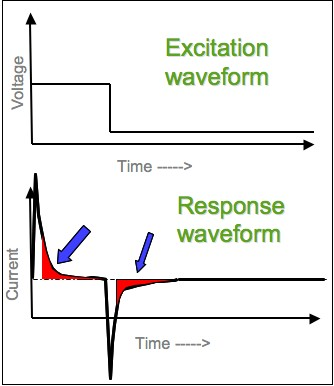
\includegraphics[scale=0.22]{CA_demo}
    \captionof{figure}{Double-pulsed chronoamperometry waveform showing
    integrated region for charge determination.\cite{CA}}
    \label{fig:CA_demo}
\end{center}
Initially, there is only a background current. When the potential is
stepped, the redox reaction quickly reaches its maximum value, then
decreases as the analyte at the eletrode's surface decreases in
concentration. \cite{myers} This relationship between the current and time can be
expressed by the Cottrell Equation, provided in Equation \ref{eq:cottrell}.
\begin{equation}
    i = \frac{nFAC\sqrt{D}}{\sqrt{\pi t}}
\label{eq:cottrell}
\end{equation}
where $i$ = current (A), $F$ = Faraday's constant (C/mol e$^-$), $A$ = area of
the electrode (cm$^2$), $D$ = diffusion coefficient (cm$^2$/s), $C$ =
concentration of the analyte in the bulk solution (mol/cm$^3$), and $t$ =
time (s).

\subsection*{Cyclic Voltammetry}
Cyclic voltammetry (CV) is the most common type of electroanalytical measurement. 
This technique involves a linear potential sweep that is then reversed in
direction, to analyze forward and backward reactions. Peak potentials and
currents and measured for the oxidation and reduction of the analytes.
Figure \ref{fig:CV_demo} illustrates a typical cyclic voltammogram and the
measurements of a fast, thermodynamically reversible reaction.
\begin{center}
    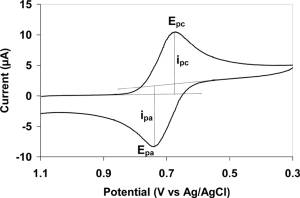
\includegraphics[scale=0.6]{CV_demo}
    \captionof{figure}{Typical cyclic voltammogram for a reversible reaction, where i$_{pc}$ and
    i$_{pa}$ show the peak cathodic and anodic current respectively.}
    \label{fig:CV_demo}
\end{center}

Thermodynamic information can also be related to the formal potential of a reaction.
Using CV, the formal potential can be calculated from the average of the peak
potentials as illustrated in Equation \ref{eq:fpot}.
\begin{equation}
    E\degree = \frac{E_{pc} + E_{pa}}{2}
    \label{eq:fpot}
\end{equation}

This is also known as the half-wave potential, and is only applicable if the
reduced and oxidized forms of a reversible redox reaction couple have
approximately equal diffusion coefficients.


\subsection*{Modes of transport}
There are three ways for an analyte to move through a solution towards an
electrode's surface: electromigration, convection, and diffusion. Electromigration is the
movement of a charged body under the influence of an electric field. In this
experiment, electromigration of the ferricyanide ion is minimized by the inclusion of a
higher concentration of supporting KCl electrolytes. The supporting electrolyte
carries the majority of the current through the solution, thus decreasing
influence of electromigration on ferricyanide. Convection is also minimized in
this experiment by keeping the sample solution still and at a constant
temperature. 

The cathodic peak current of a first forward pass of a diffusion-controlled,
reversible CV can be described by the Randles-Sevcik equation, given in Equation
\ref{eq:RS} at 25$\degree$C.
\begin{equation}
    i_{pc} = kAC\sqrt{n^3Dv} 
    \label{eq:RS}
\end{equation}
where $i_{pc}$ is the peak current (A), $k$ is a constant (2.69 $\times$ 10$^5$
C mol$^{-1}$ V$^{-1/2}$), $A$ is the electrode area (cm$^2$), $C$ is the
concentration of the reacting species in solution (mol L$^{-1}$), $n$ is the
number of electrons involved in the reaction, $D$ is the diffusion coefficient
for the reacting species (cm$^2$ s$^{-1}$), and $v$ is the potential sweep rate
(Vs$^{-1}$).

\section*{Experimental}
\subsection*{Instrumental Parameters}
A three-electrode cell was used in this experiment.
A Ag|AgCl reference electrode was used, with a Ag wire suspended in a saturated
solution of KCL and AgCl. A platinum wire was used as the auxiliary electrode,
and a 1.7 mm diameter platinum disk was used as the working electrode.
For measuring the thyronine reactions, a 1.7 mm diameter glassy carbon
electrode was used for its affinity with thyronine and its side products.
Figure \ref{fig:potentiostat} provides an illustration of the
three-electrode cell used in this study.
\begin{center}
    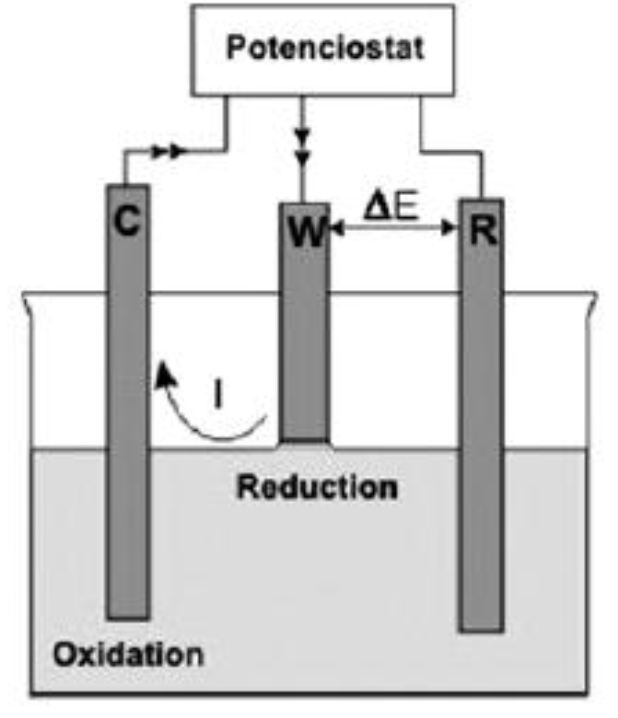
\includegraphics[scale=0.3]{potentiostat}
    \captionof{figure}{Schematic representation of the electrochemical cell
    used in this study. C indicates the auxilliary electrode, W indicates
    the working electrode, and R indicates the reference electrode.}
    \label{fig:potentiostat}
\end{center}

A CHI603 Electrochemical Analyzer by CH Instruments, Inc. was used to
monitor and analyze current flow.
A range of potentials from 0.1 V to 0.45 V was used in running
chronoamperometry.
Cyclic voltammetry runs on ferricyanide were conducted using a range of potentials from 0.0 V to
0.5 V.
CV runs on the unknown solutions were conducted using a rage of potentials from
0.0 V to 1.2 V.

\subsection*{Sample Preparation}
A 1 M solution of H$_2$SO$_4$ in high purity H$_2$O was used in cleaning the
sample vial and for making the necessary solutions. 
Care was given to not mix the Fe(CN)$_6$ solutions with the acidic solutions.
A 50 mL solution of 5 $\times$ 10$^{-3}$ M K$_3$[Fe(CN)$_6$] and 1 M KCl in H$_2$O was prepared.
A mass of 0.0830 g of K$_3$[Fe(CN)$_6$] and 3.7263 g of KCl was used.
The electrodes were polished and cleaned prior to each run. 
A chronoamperomagram was run on Fe(CN)$_6$ solution. Cyclic voltammograms were
then generated of the Fe(CN)$_6$ solution for scan rates of 0.1, 0.075, 0.05,
and 0.025 V/s.
The three unknown solutions were diluted to 25 mL with the 1 M H$_2$SO$_4$ solution.
Cyclic voltammograms were then run on the unknown samples at a scan rate of 0.1
V/s. 

\section*{Results}
According to literature, the diffusion coefficient of [Fe(CN)$_6$]$^{3-}$ is
7.63 $\times$ 10$^{-6}$ cm$^2$s$^{-1}$ in 0.1 M KCl. \cite{trau} 
The results of this experiment are deemed precise, accurate, and reproducible.

Table \ref{tab:res} provides the results of this experiment.
\begin{center}
    \captionof{table}{Tabulated data of experimental results.}
    \begin{tabular}{l|c}
        \hline
        Formal reduction potential E$\degree$ (V) & 0.273 \\
        Experimental half-wave potential E$_{1/2}$ (V) & 0.2531 $\pm$ 0.0004 \\
        Number of e$^-$ in redox process (mol) & 1 $\pm$ 1 \\
        Diffusion coefficient (Cottrell) (cm$^2$/s) & 2.56 $\times$ 10$^{-5}$ \\
        Diffusion coefficient (Randles-Sevcik) (cm$^2$/s) & 8.38 $\times$ 10$^{-6}$ \\
    \end{tabular}
    \label{tab:res}
\end{center}

Figure \ref{fig:CA} shows the chronoamperogram of the Fe(CN)$_6$ solution.
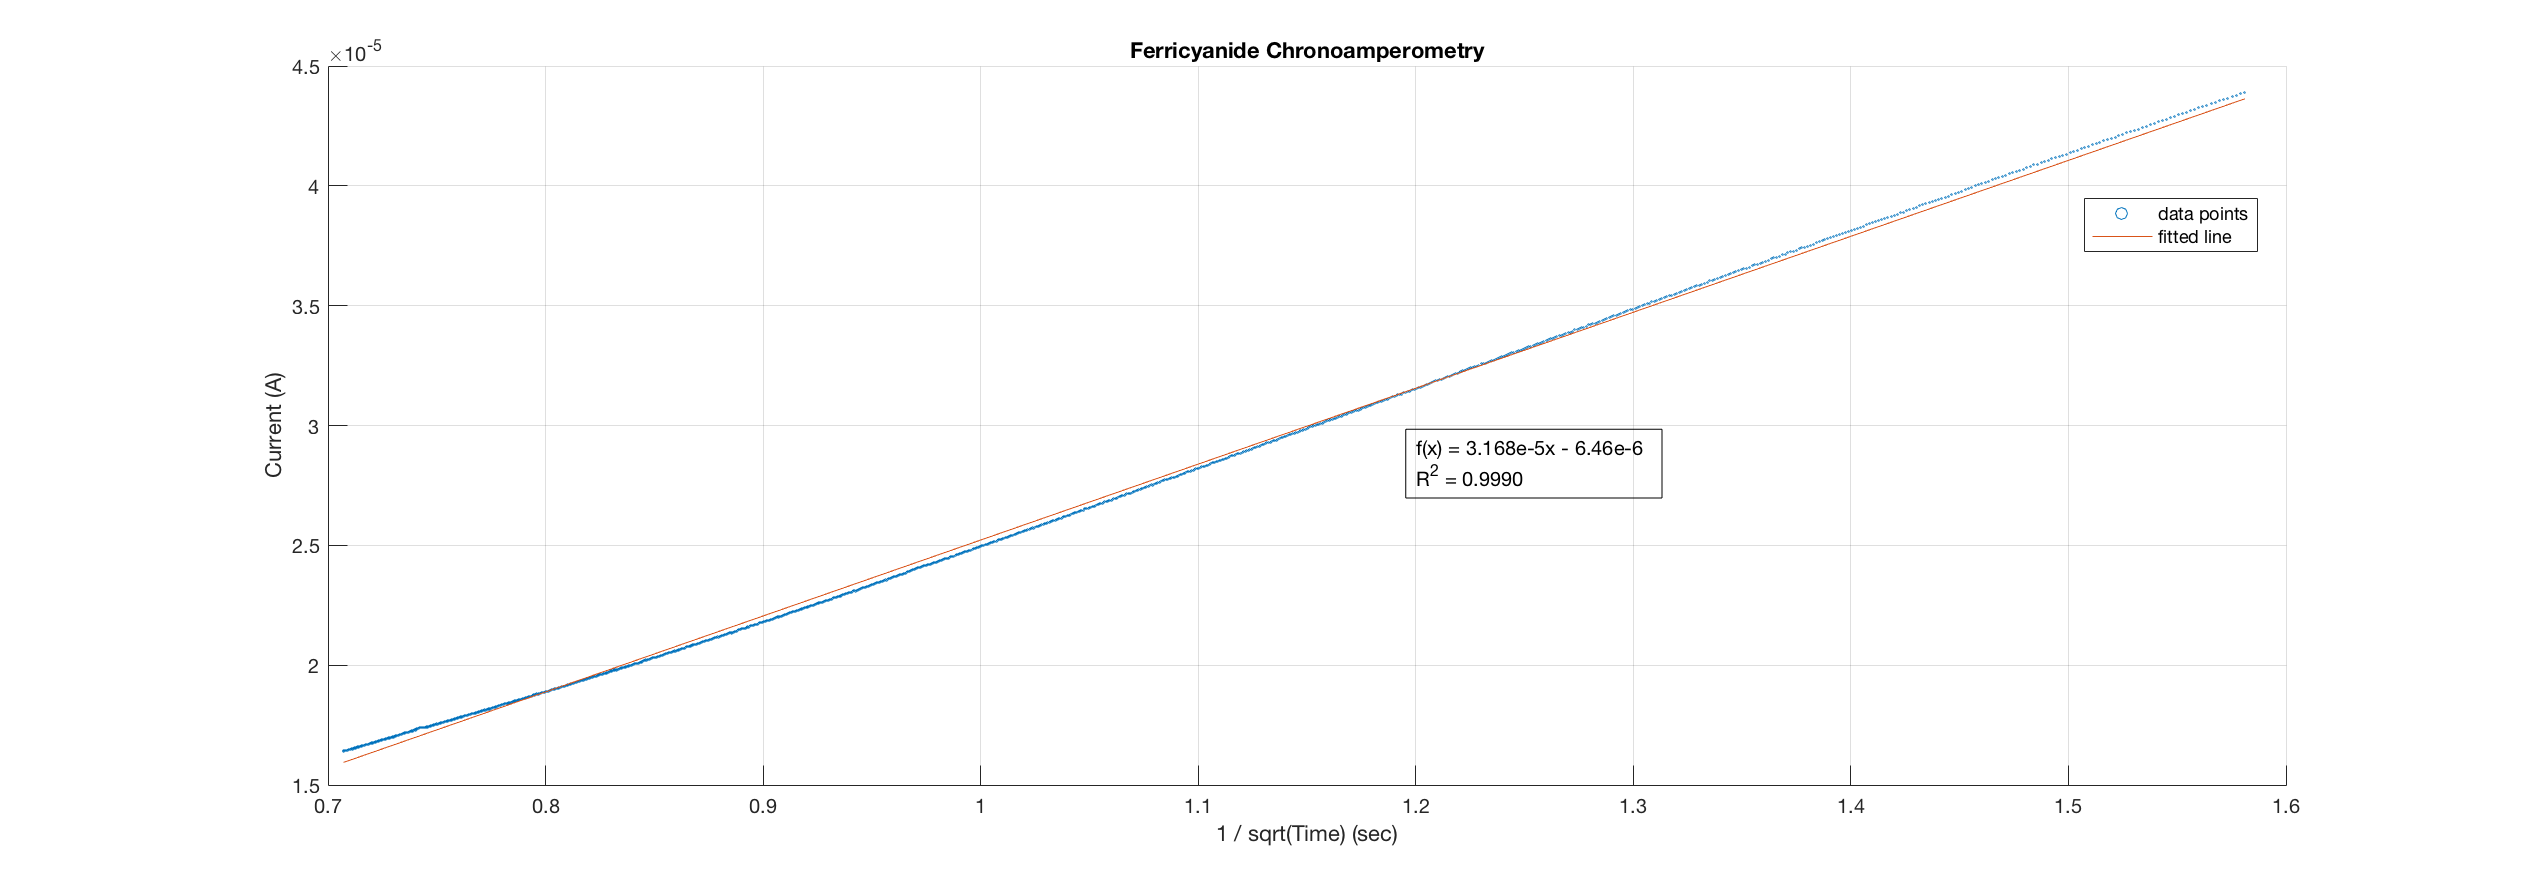
\includegraphics[scale=0.1]{CA}
    \captionof{figure}{Chronoamperometry plot of Fe(CN)$_6$.}
    \label{fig:CA}

Figure \ref{fig:E_pc} shows Cottrell's plot of the Fe(CN)$_6$ solution.
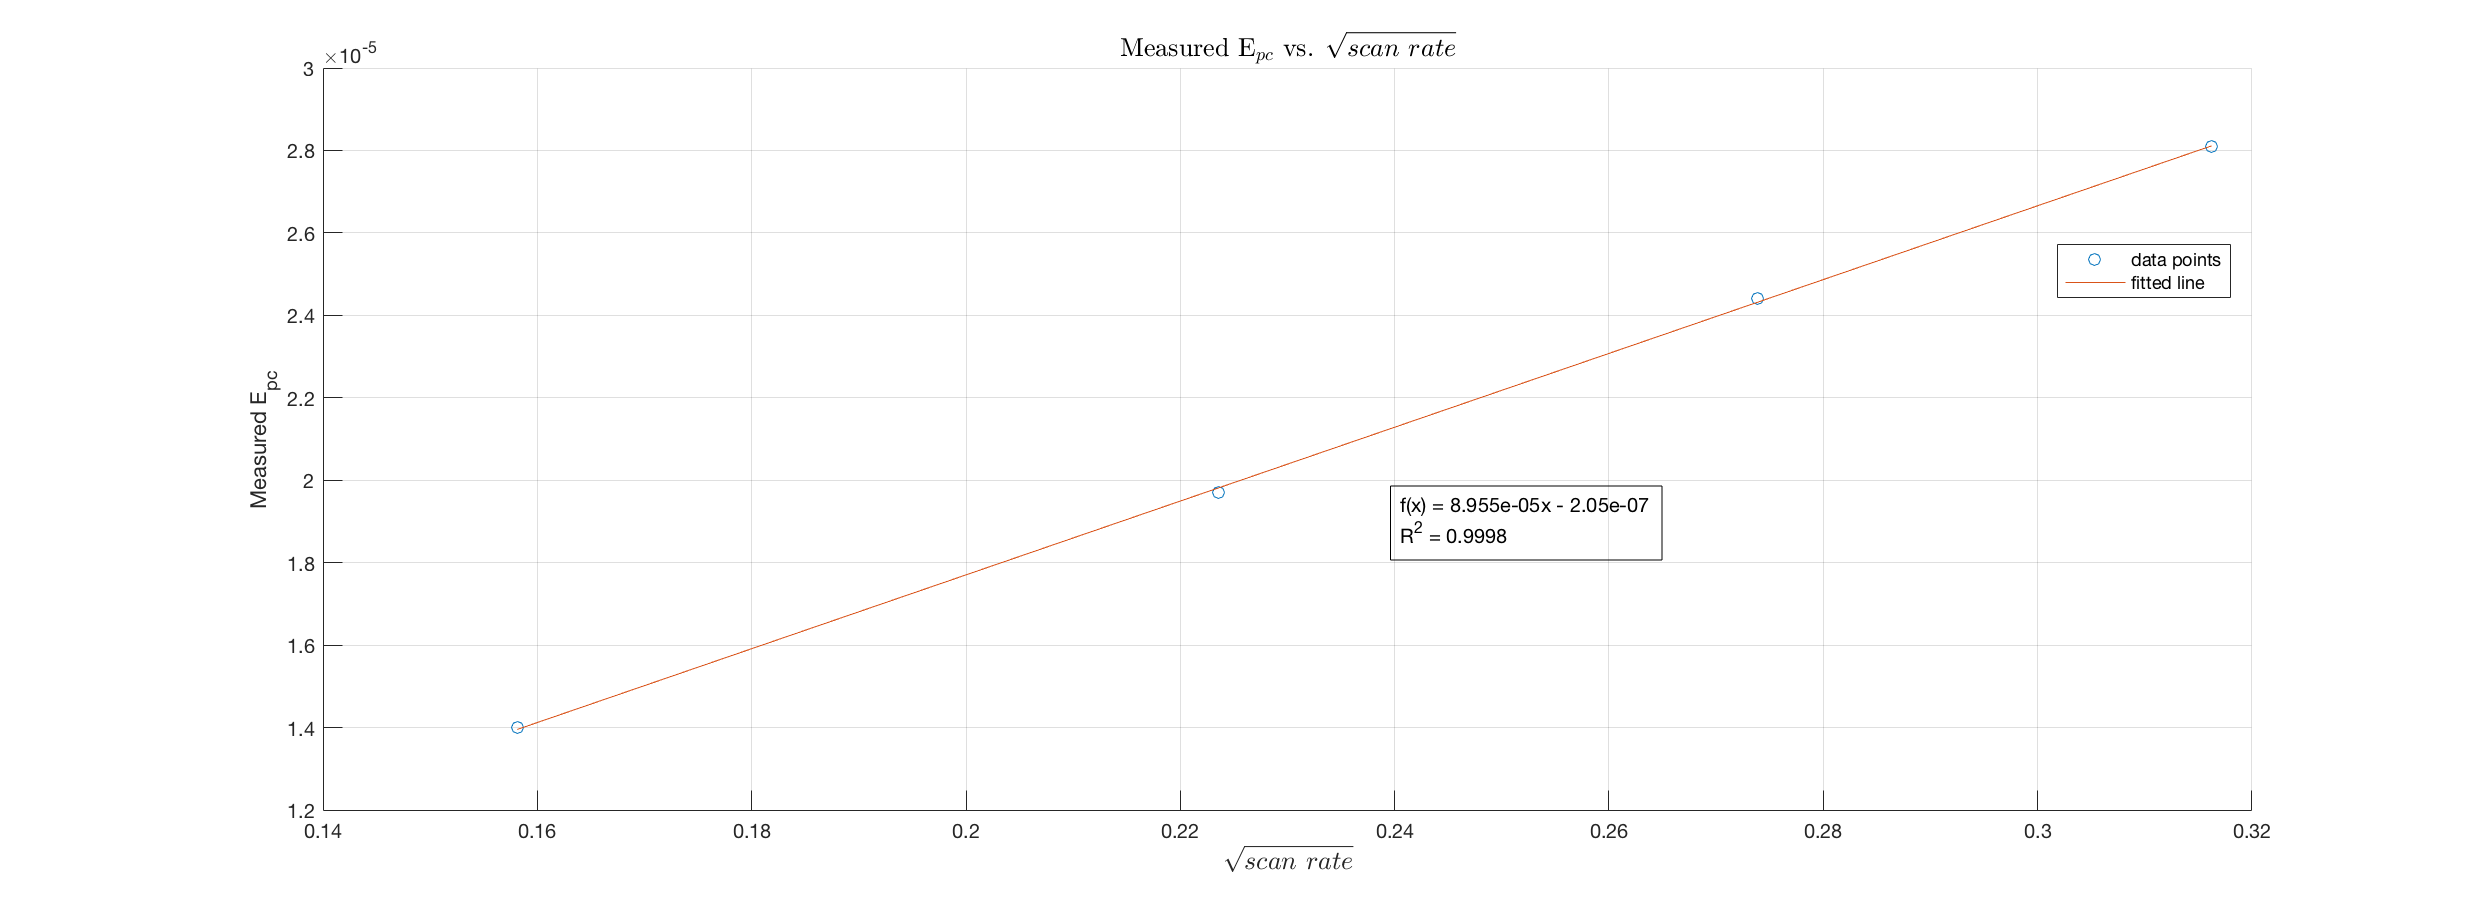
\includegraphics[scale=0.1]{E_pc}
    \captionof{figure}{Cottrell's plot for potential step chronoamperometry of
    Fe(CN)$_6$.}
    \label{fig:E_pc}

Figure \ref{fig:FeCN_CV} shows a cyclic voltammogram of the Fe(CN)$_6$ solution.
\begin{center}
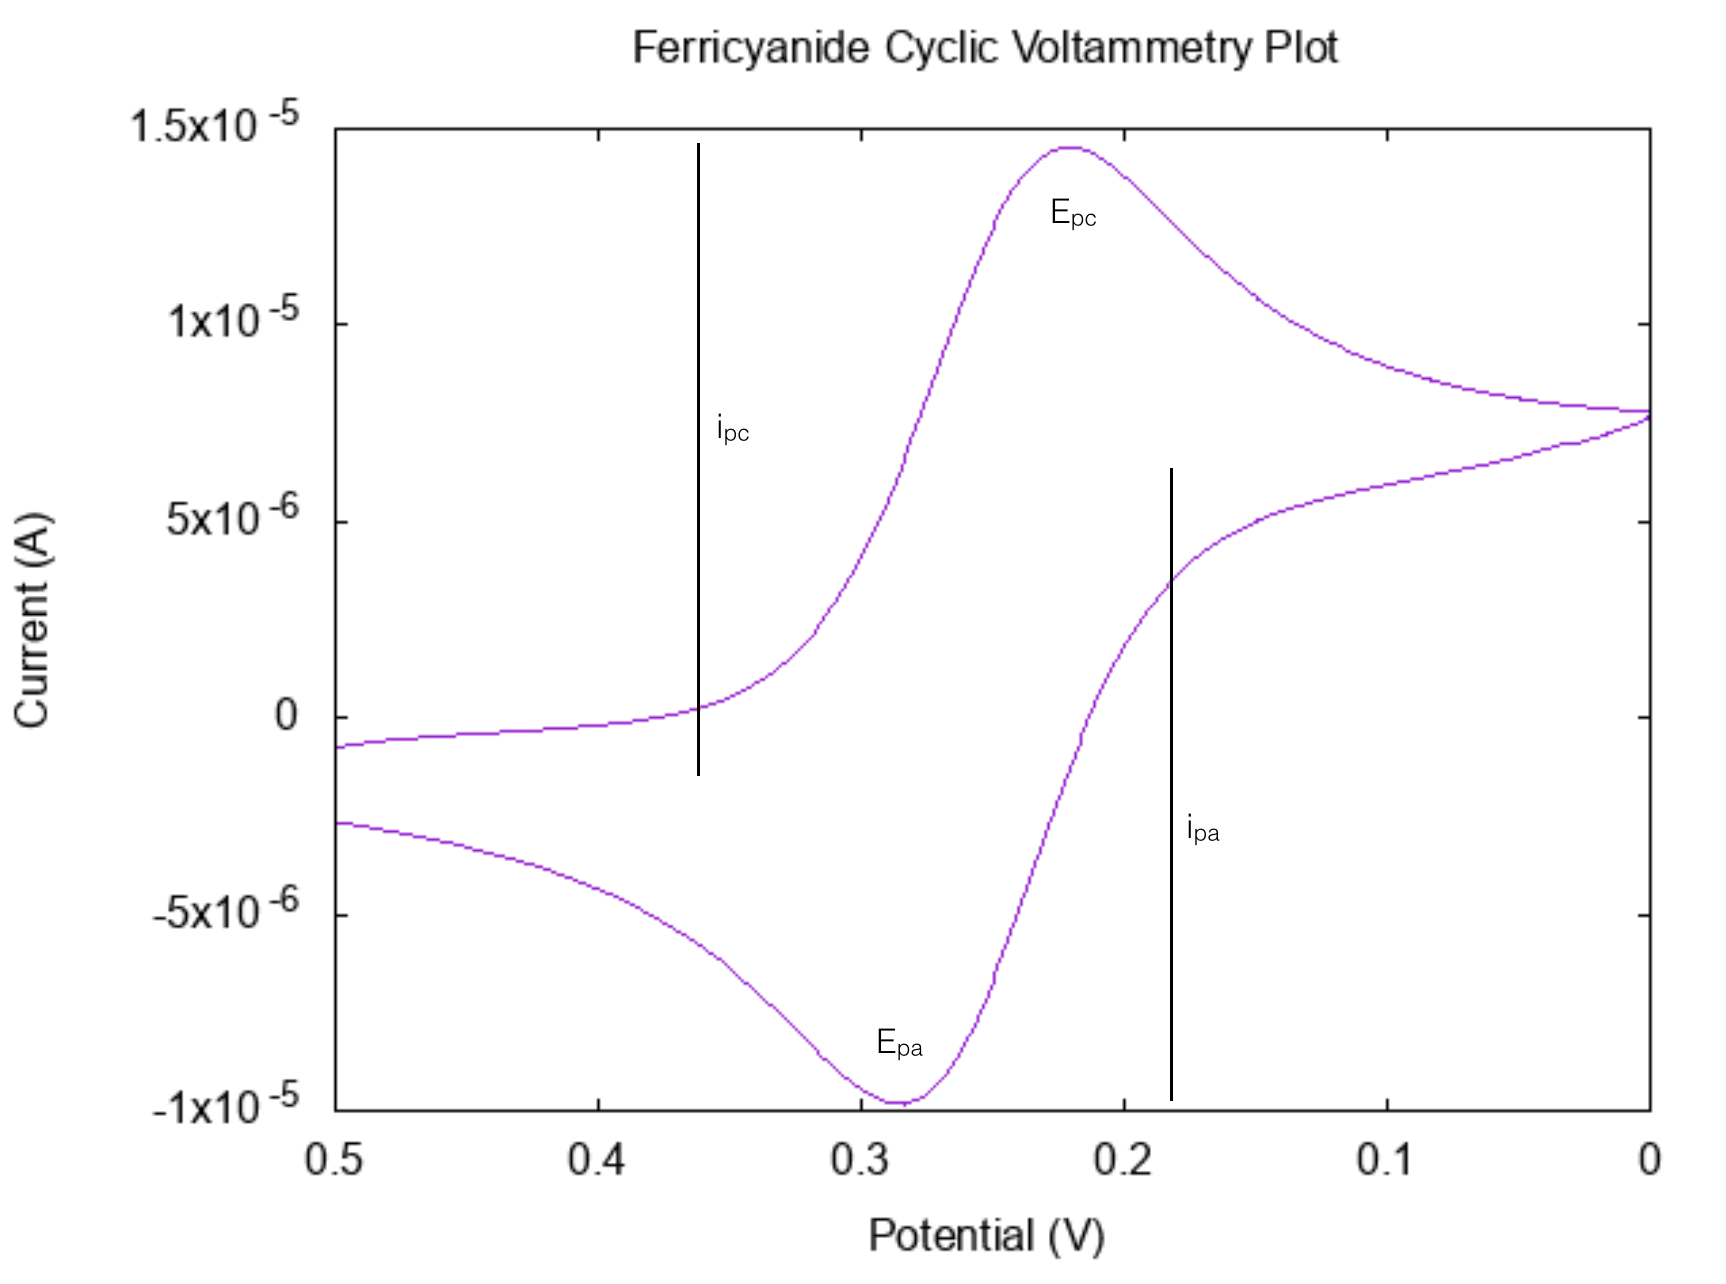
\includegraphics[scale=0.2]{FeCN_CV}
    \captionof{figure}{Cyclic voltammery plot of Fe(CN)$_6$ with 0.025 V/s scan rate.}
    \label{fig:FeCN_CV}
\end{center}


\section*{Discussion}
The results obtained in this experiment are within expected values,
however, precision may be improved with the inclusion of more sample runs under
varying scan rates and parameters. 
While electromigration and convection variables have been minimized in this
experiment, it is inevitable that they still play some part in the outcome of
the results. For the purposes of this experiment, electromigration and
convection variables are assumed to be 0 and are not factored into consideration
in determining the results and diffusion coefficients.

[1a] Figure \ref{fig:CA_dis} shows a typical signal graph of a chronoamperometry
run. In region a, the potential is held constant at a value typically higher
than the reduction potential of the analyte being measured. No reaction is
occuring at this potential.
In region b, the potential is stepped to a lower potential than the analyte reduction
potential, causing any molecules that come into contact with the electrode to be
reduced. A high current is initially observed due to the fast reaction rate and high
initial concentration of reducible ions present near the electrode. 
Over time, the current will drop as the concentration of reducible ions near the
electrode decreases, as seen in region c.
\begin{center}
    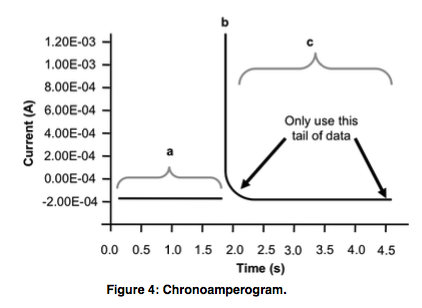
\includegraphics[scale=0.4]{CA_dis}
    \captionof{figure}{A typical chronoamperogram.}
    \label{fig:CA_dis}
\end{center}
[1b] Figure \ref{fig:CV_dis} shows a typical signal graph of a cyclic
voltammogram. In region a, the CV scan begins at a potential above the reduction
potential of the analyte being measured. As the potential is linearly decreased,
the current will begin to flow once the potential is low enough to begin the
reduction reaction, as seen in region b. The current will continue to increase
until it reaches the peak cathodic current at region c, where the concentration
reducible ions approaches 0. After the depletion of reducible ions, the current
will begin to decrease, as seen in region d. 
Now, the scanning direction is reversed, so that the potential is increased.
This increase in potential also causes an increase in the oxidation reaction of
the chemical species, and results in a increase in current as seen in region e.
This oxidation continues until the anodic peak current is reached at region f,
as the amount of oxidizable species approaches 0. 
The current then continues to drop, as the amount of oxidizable species becomes
depleted near the electrode's surface, as seen in region g.
\begin{center}
    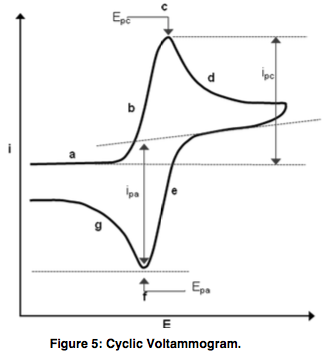
\includegraphics[scale=0.4]{CV_dis}
    \captionof{figure}{A typical cyclic voltammogram.}
    \label{fig:CV_dis}
\end{center}

[2] The experimentally determined number of electrons participating in the
redox reactions of ferricyanide is 1. This is in agreement with the redox reactions
attributed to the anodic and cathodic peaks.

[3a] The diffusion coefficient is a propotionality constant between the molar
flux as a result of molecular diffusion and the concentration gradient of the
species. [3b] In this experiment the diffusion coefficient of
[Fe(CN)$_6$]$^{3-}$ was determined. 
A value of 2.56 $\times$ 10$^{-5}$ cm$^2$/s was found using the Cottrell
equation.
A value of 8.38 $\times$ 10$^{-6}$ cm$^2$/s was found using the Randles-Sevcik
equation.
Both values are relatively close to each other, and are comparatively accurate
against literature values. \cite{trau}

[4a] Stirring of the sample solution would cause the experimentally observed
peak heights to increase due to increased rate of contact of the
reducible/oxidizable species against the electrode. This increased rate of
contact and electron exchange would cause an increase in the measured current
peak.  
[4b] In this experiment, movement of the ferricyanide ions by convection
was minimized by keeping the solution still and at room temperature. This
allows for the analytical measurement of the diffusion coefficient with minimal
interference from other movement variables such as convection and
electromigration.

[5a] The unknown samples for A, B, and C are Benzoquinone, Thyronine, and
Tyrosine respectively.
[5b,c] See Appendix for labeled voltammograms of each unknown.
[5d] Benzoquinone is the only species that follows a singular, reversible redox
reaction. The cyclic voltammogram of Sample A follows this pathway, therefore
Sample A is benzoquinone.
Thyronine undergoes an oxidation reaction, that produces two products following
hydrolysis. This would equate to 3 anodic peaks, which the cyclic voltammogram
of Sample B has.
Finally, Tyrosine irreversibly undergoes an oxidation reaction. This is
represented by the singular anodic peak on the cyclic voltammogram of Sample C.
Therefore, Sample C is Tyrosine.


\subsection*{Literature Review}
A refereed article that uses cyclic voltammetry to determine diffusion
coefficients is the "Voltammetry of Oxygen in the Room-Temperature Ionic Liquids
1-Ethyl-3-methylimidazolium Bis((trifluoromethyl)sulfonyl)imide and
Hexyltriethylammonium Bis((trifluoromethyl)sulfonyl)imide:  One-Electron
Reduction To Form Superoxide. Steady-State and Transient Behavior in the Same
Cyclic Voltammogram Resulting from Widely Different Diffusion Coefficients of
Oxygen and Superoxide". \cite{oxy}
In this study, the electrochemical reduction of oxygen in two different ionic
liquids was investigated. The diffusion coefficients of O$_2$ and O$_2^{*-}$ in
[N$_{6222}$][N(Tf)$_2$] was found to be 1.48 $\times$ 10$^{-10}$ m$^2$/s and
4.66 $\times$ 10$^{-12}$ m$^2$/s respectively.
The diffusion coefficients of O$_2$ and O$_2^{*-}$ in [EMIM][N(Tf)$_2$] was
found to be 7.3 $\times$ 10$^{-10}$ m$^2$/s and 2.7 $\times$ 10$^{-10}$ m$^2$/s
respectively.
A gold microdisk working electrode was used in this study.

\section*{Conclusion}
The diffusion coefficient of [Fe(CN)$_6$]$^{3-}$ was found to be 2.56 $\times$
10$^{-5}$ cm$^2$/s from the Cottrell equation, and 8.38 $\times$ 10$^{-6}$
cm$^2$/s from the Randles-Sevcik equation in 1 M KCl. As compared to literature
values \cite{trau}, these results are deemed reasonable.

Sources of error may include random error on the part of the preparation of the
samples, as multiple people were involved in the process. Systematic error in
the handling of the electrochemical cell and analyzing instrument may also have
been a factor. These sources of error may cause a loss of precision in
determining cathodic and anodic peaks, resulting in incorrect calculations of
diffusion coefficients.

\bibliography{elec.bib}

}
\end{multicols}

\newpage
\section*{Appendix}
\begin{enumerate}
    \item Chronoamperogram of Fe(CN)$_6$ solution.
    \item Cottrell's plot for potential step chronoamperometry of Fe(CN)$_6$
        solution.
    \item Cyclic voltammogram of Fe(CN)$_6$ solution with 0.025 V/s scan rate.
    \item Cyclic voltammogram of unknown Samples A, B, and C.
    \item Reduction and oxidation reactions of thyronine, tyrosine, and
        benzoquinone.
    \item Laboratory notebook pages with raw data.
\end{enumerate}

\newpage
\begin{center}
    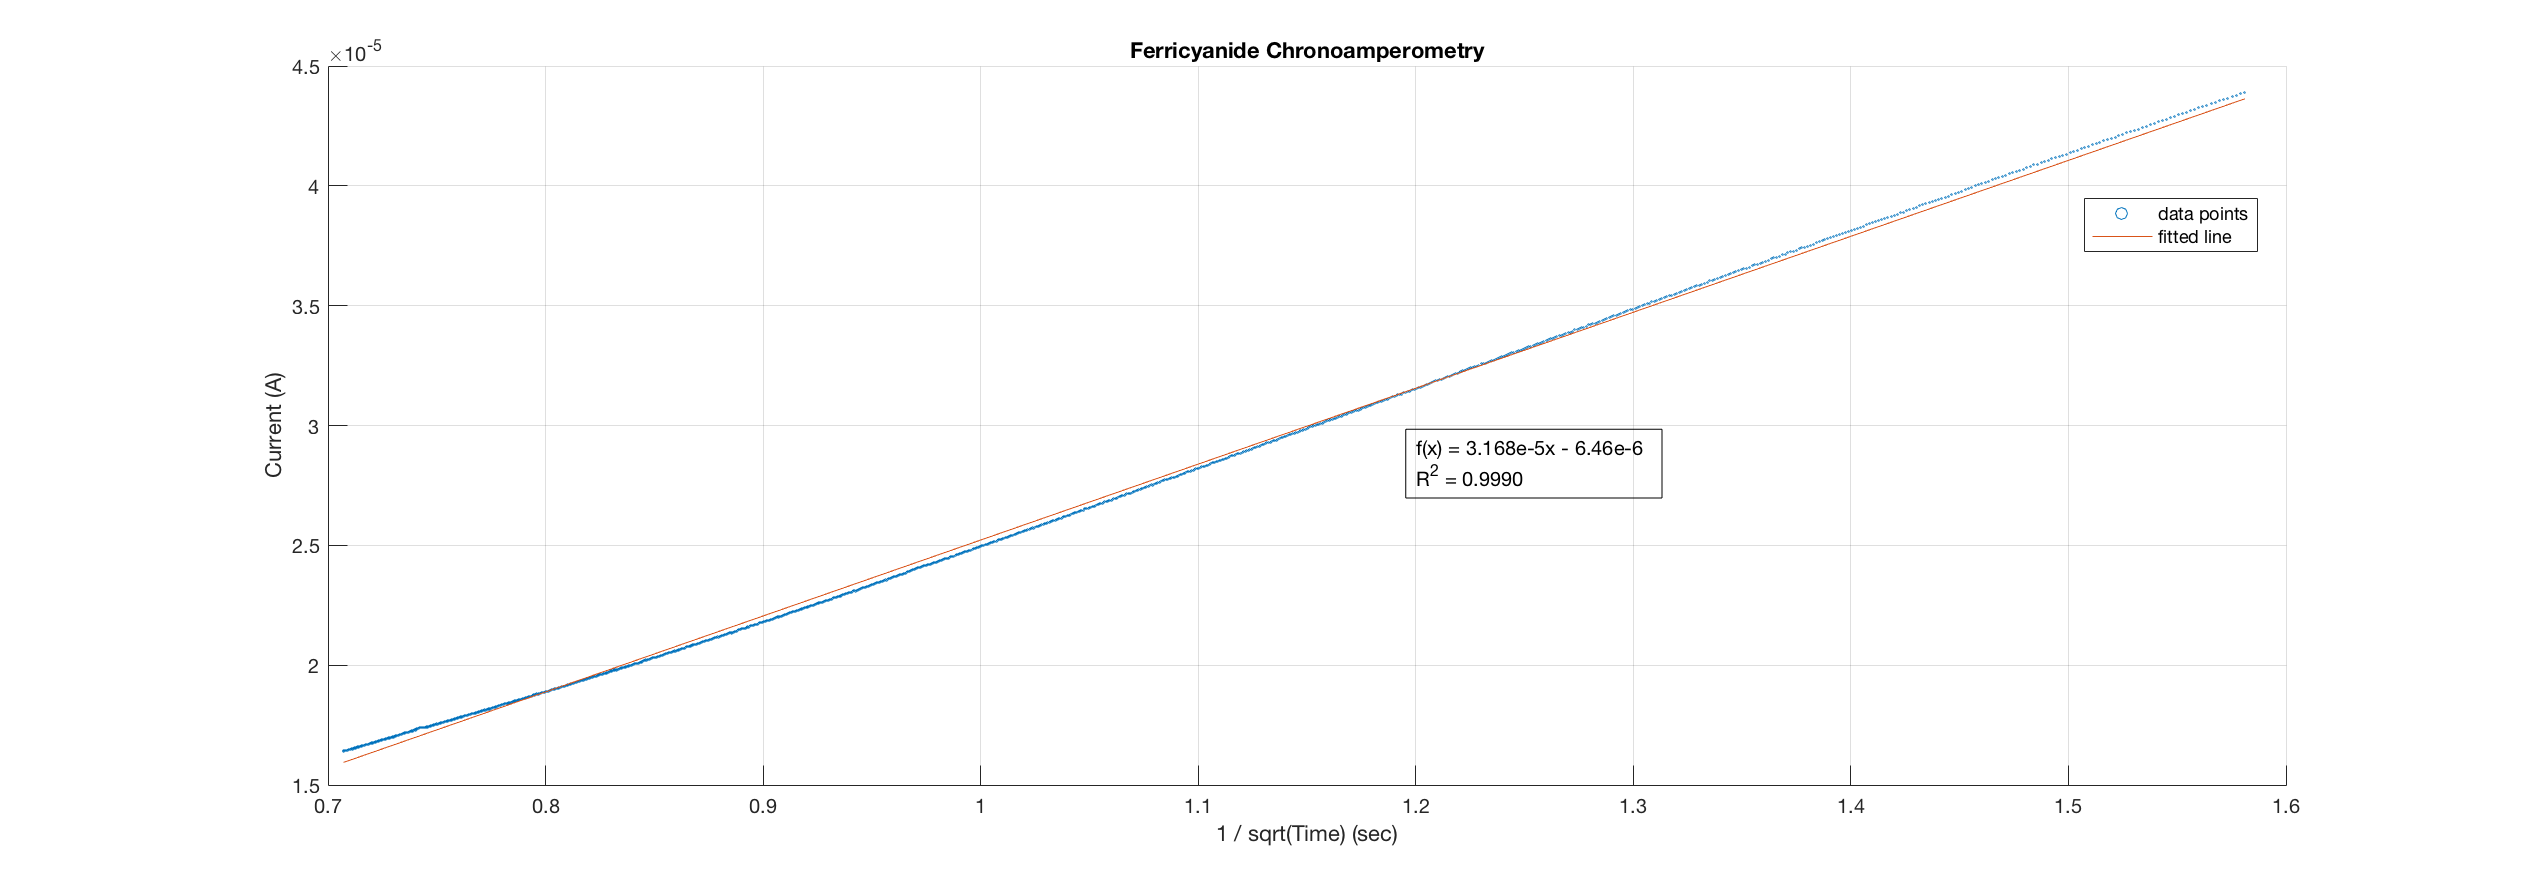
\includegraphics[scale=0.18]{CA}
    \captionof{figure}{Chronoamperometry plot of Fe(CN)$_6$.}
    \vspace{5cm}
    
    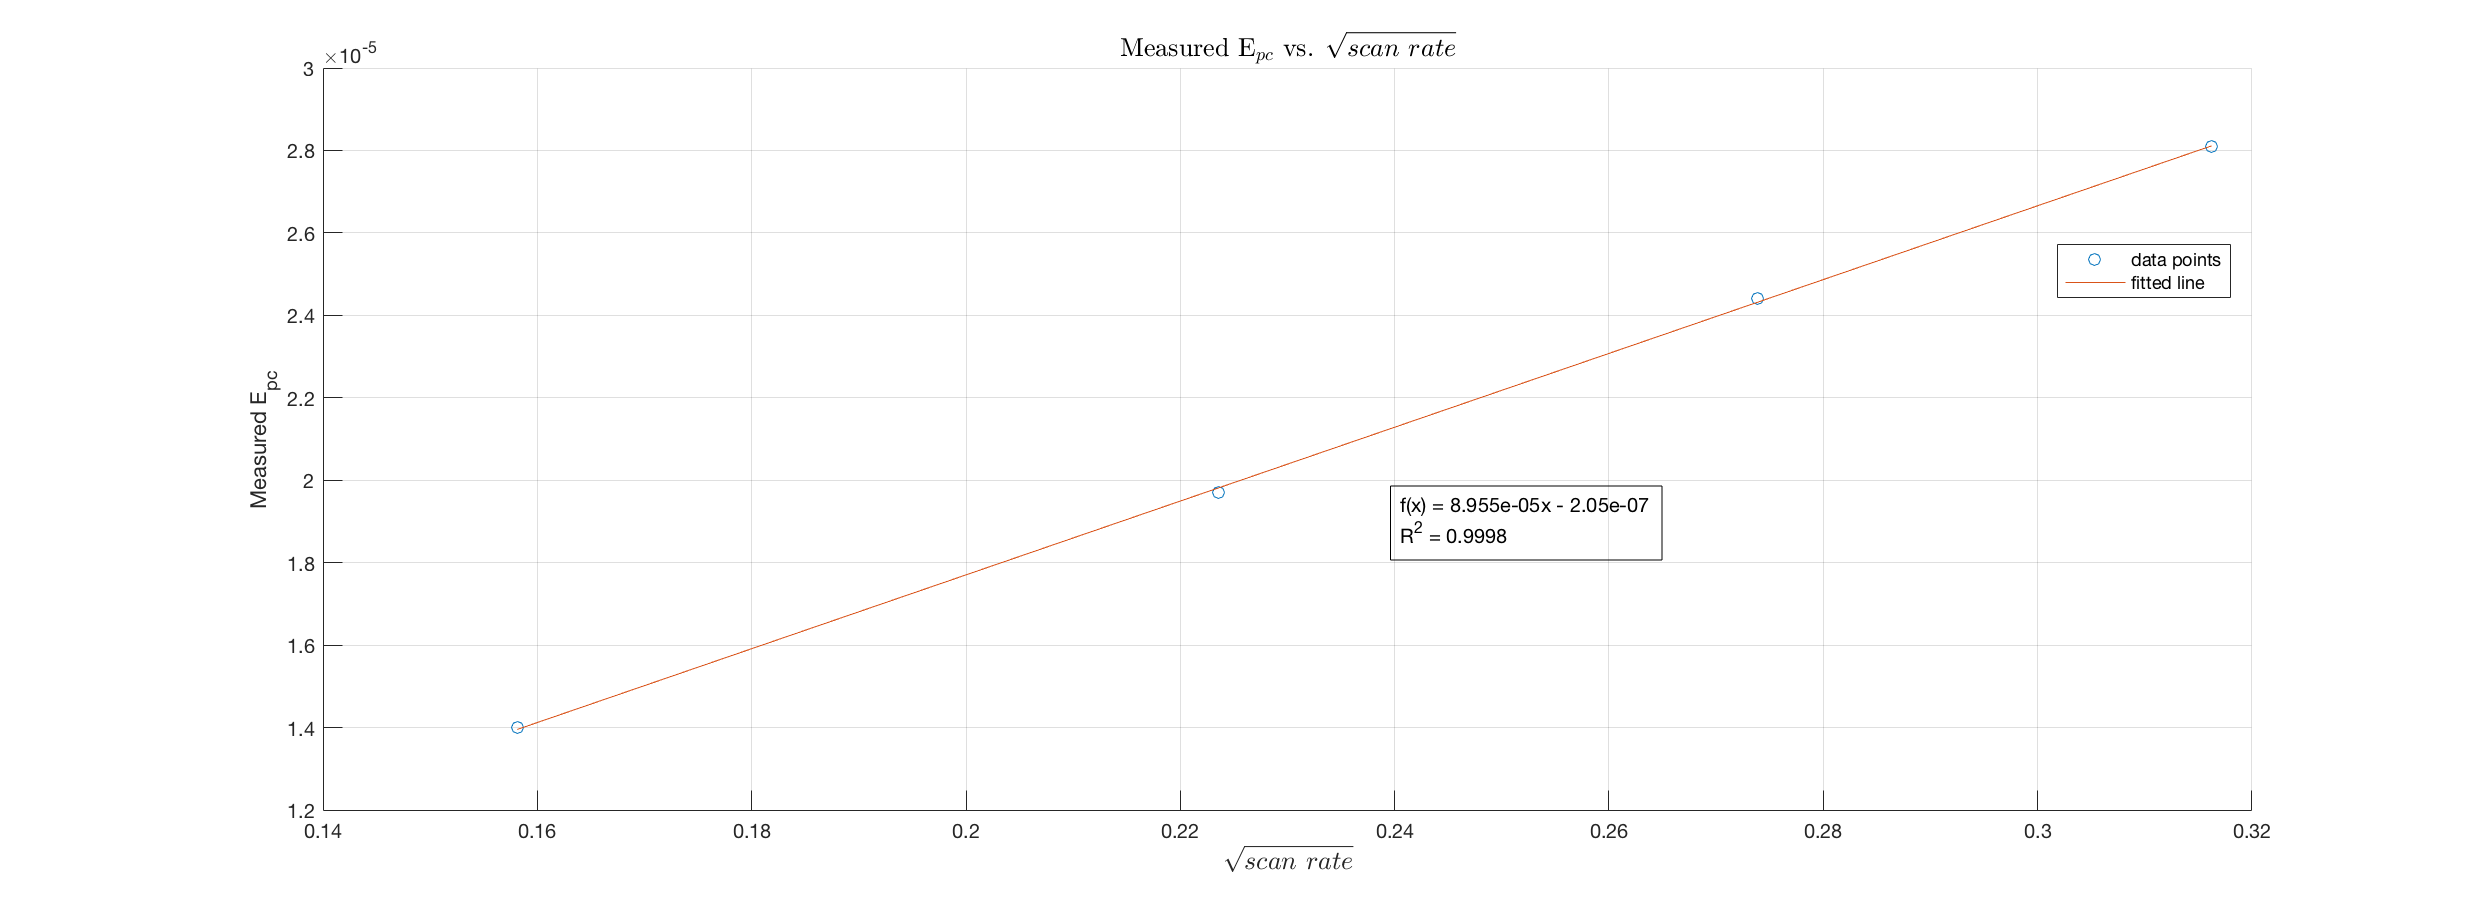
\includegraphics[scale=0.18]{E_pc}
    \captionof{figure}{Cottrell's plot for potential step chronoamperometry of
    Fe(CN)$_6$.}

    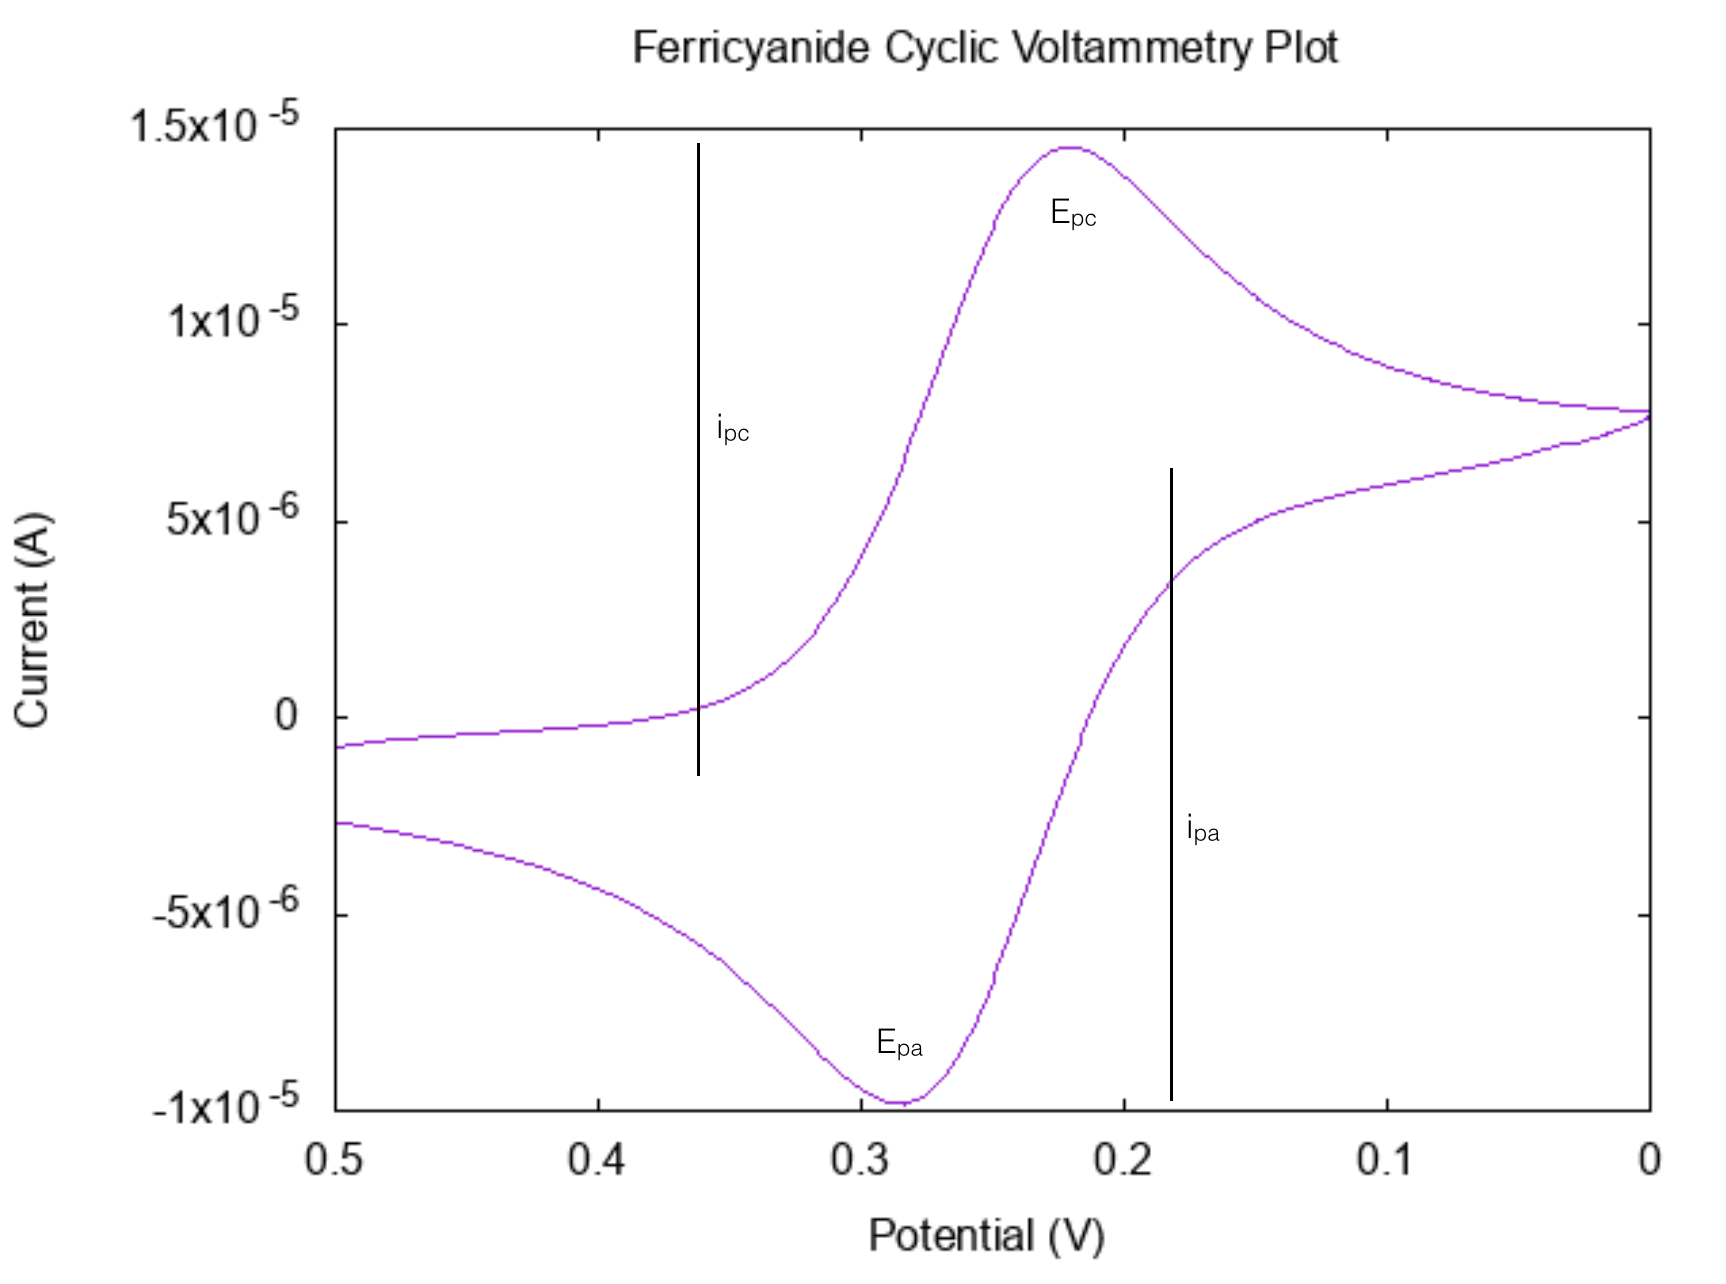
\includegraphics[scale=0.4]{FeCN_CV}
    \captionof{figure}{Cyclic voltammery plot of Fe(CN)$_6$ with 0.025 V/s scan rate.}
    \vspace{5cm}

    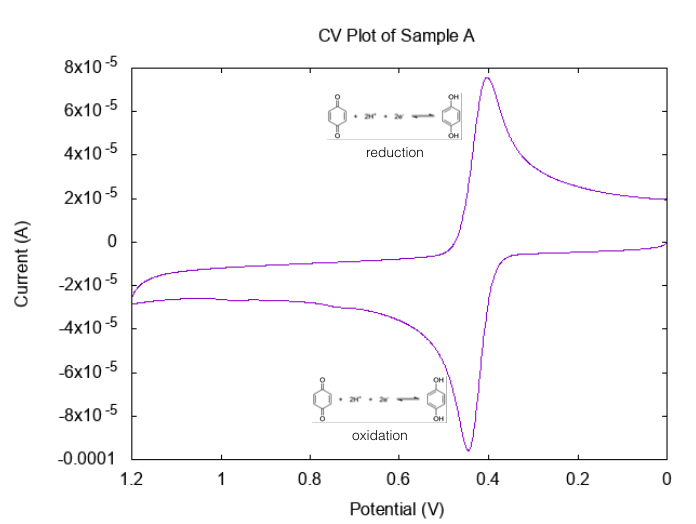
\includegraphics[scale=0.7]{SampleA}
    \captionof{figure}{Cyclic voltammetry plot of unknown Sample A, Benzoquinone.}
    \vspace{2cm}

    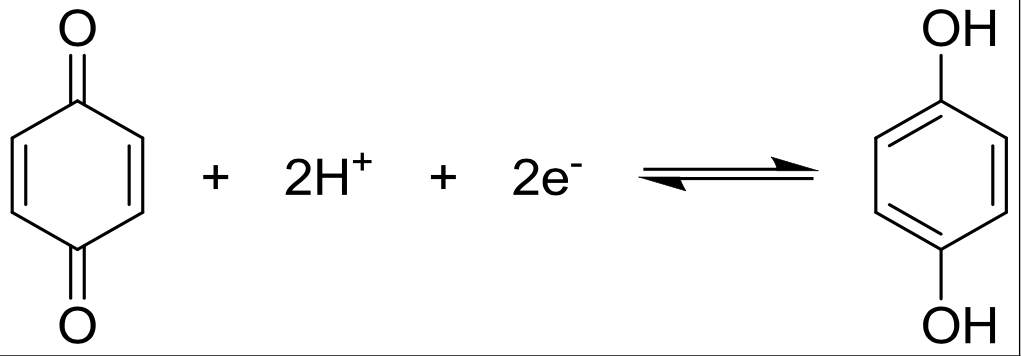
\includegraphics[scale=0.5]{benzoquinone}
    \captionof{figure}{Benzoquinone: reduction / p-hydroquinone oxidation
    (reversible).\cite{lab_man}}


    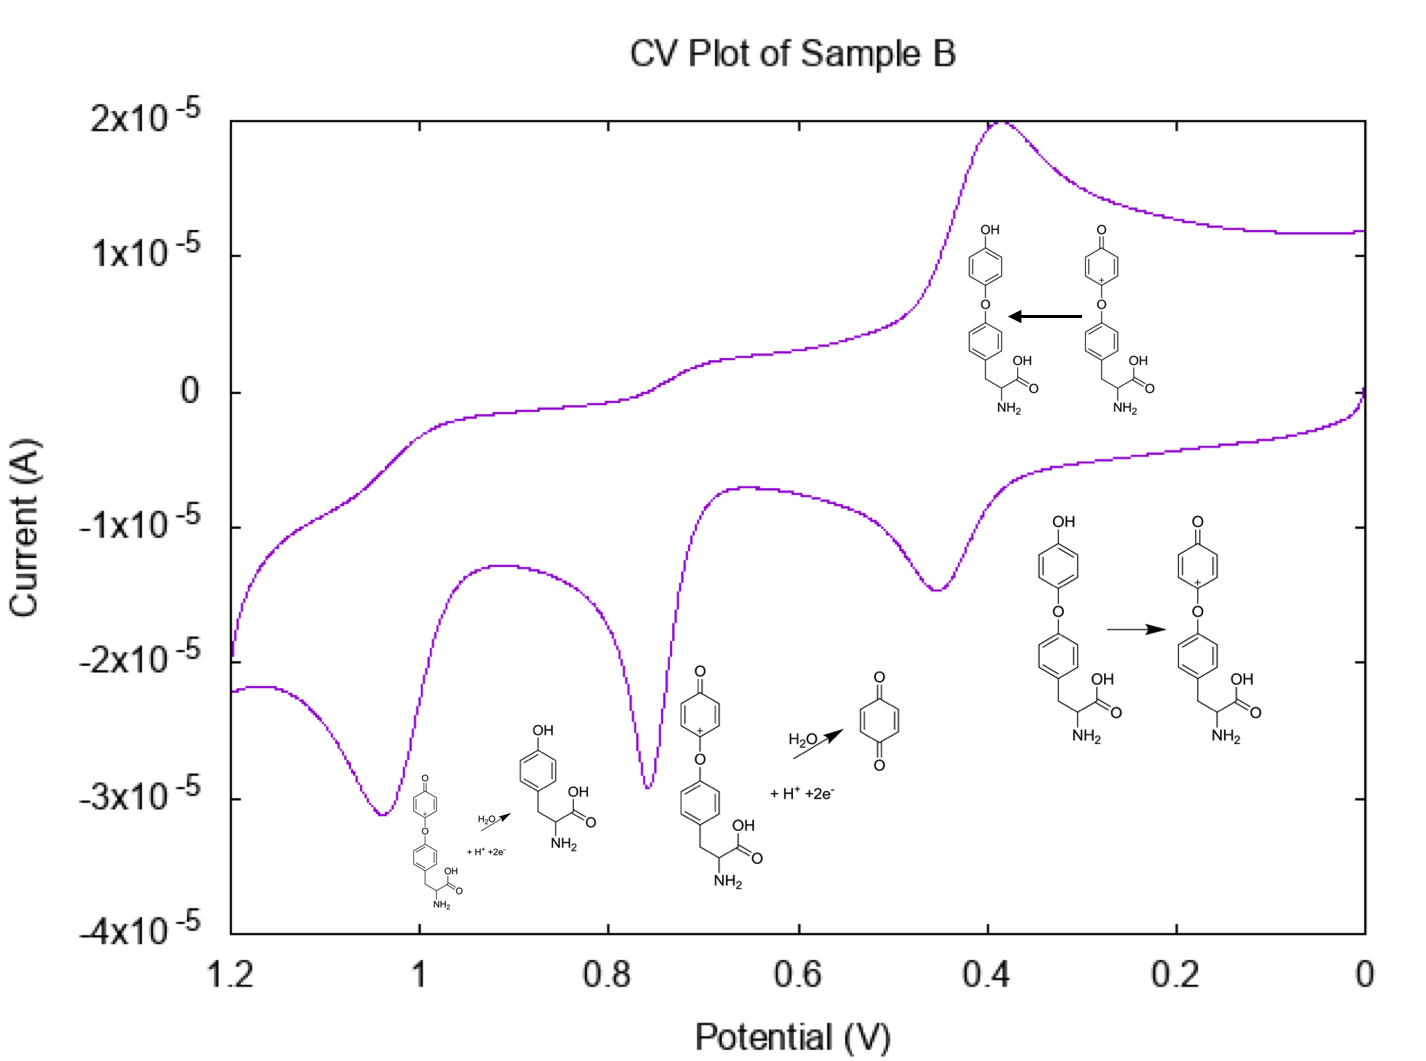
\includegraphics[scale=0.3]{SampleB}
    \captionof{figure}{Cyclic voltammetry plot of unknown Sample B, Thyronine.}
    \vspace{2cm}

    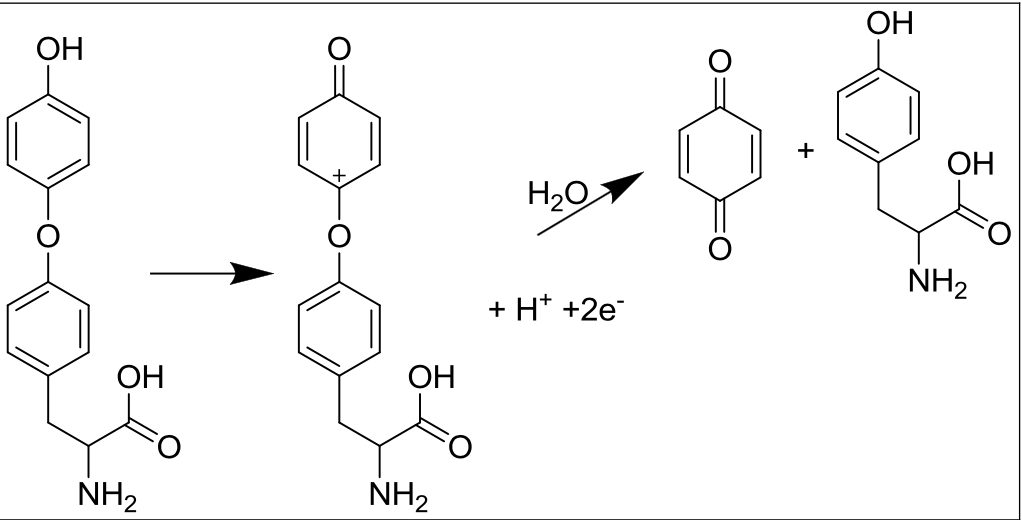
\includegraphics[scale=0.5]{thyronine}
    \captionof{figure}{Thyronine: oxidation followed by a hydrolysis (making
    tyrosine and benzoquinone).\cite{lab_man}}
    \vspace{2cm}


    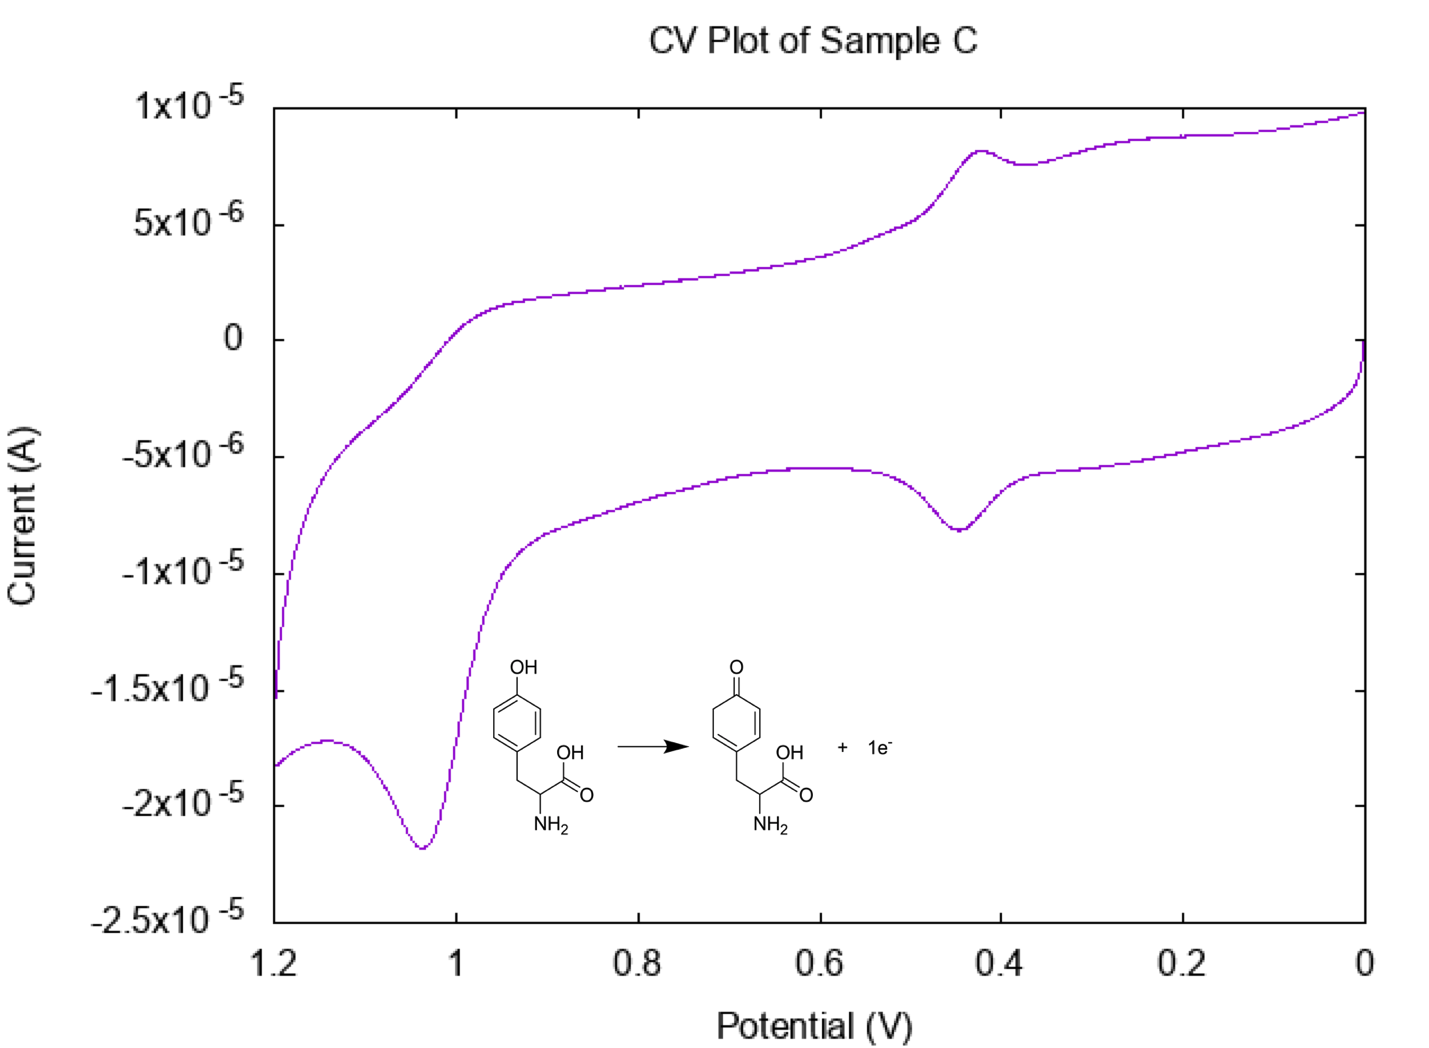
\includegraphics[scale=0.3]{SampleC}
    \captionof{figure}{Cyclic voltammetry plot of unknown Sample C, Tyrosine.}
    \vspace{2cm}

    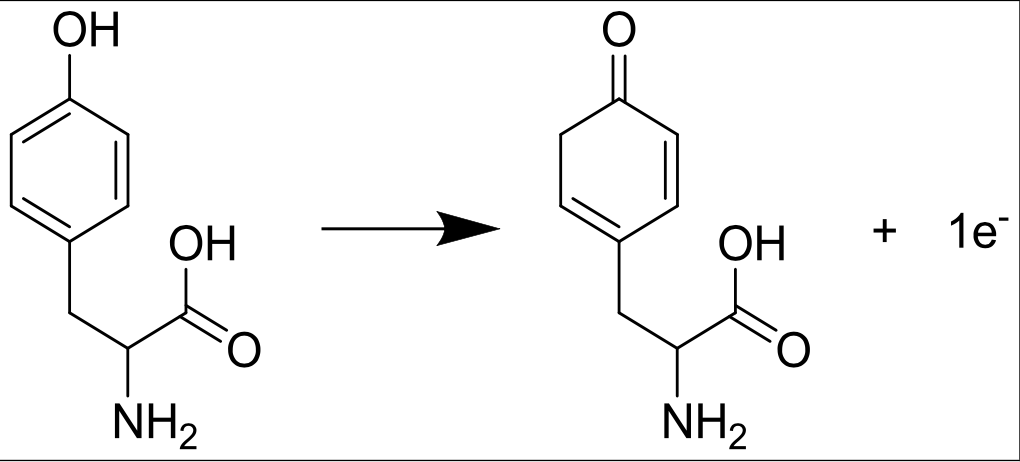
\includegraphics[scale=0.5]{tyrosine}
    \captionof{figure}{Tyrosine: oxidation (irreversible).\cite{lab_man}}

\newpage 
\subsection*{Sample Calculations on Determining the Diffusion Coefficient
of [Fe(CN)$_6$]$^{3-}$ by Cottrell's Equation}
\vspace{2cm}

Cottrell's Equation is given below:
\begin{equation*}
    i = \frac{nFAC\sqrt{D}}{\sqrt{\pi t}} 
\end{equation*}

where F = 96484.6 C/mol \\
    n = 1 mol e$^-$ \\
    A = 0.023 cm$^2$ \\
    C = 5 $\times$ 10$^{-6}$ mol/mL \\
\vspace{1cm}
the slope of the line of best fit found from the generated Cottrell's plot is $m = 3.168 \times
    10^{-5}$.

Rearranging the equation gives:
    \begin{equation*}
        m = \frac{nFAC\sqrt{D}}{\sqrt{\pi}}
    \end{equation*}

    \begin{equation*}
        D = \frac{m^2 \pi}{n^2F^2A^2C^2}
    \end{equation*}

    \begin{equation*}
        D = 2.56 \times 10^{-5}
    \end{equation*}

\end{center}
\end{document} 
